\documentclass[11pt,a4paper]{article}
\usepackage[utf8]{inputenc}
\usepackage[german]{babel}
\usepackage[T1]{fontenc}
\usepackage{amsmath}
\usepackage{amsfonts}
\usepackage{amssymb}
\usepackage{graphicx}
\usepackage[export]{adjustbox}
\usepackage{float}
\usepackage{subcaption}
\usepackage{caption}

\begin{document}

\begin{titlepage}
\newcommand{\HRule}{\rule{\linewidth}{0.5mm}}
\center

\includegraphics[scale=0.075]{tuchem.png} \\[1cm]
\textsc{\LARGE
Entwicklerhandbuch
} \\[1cm]
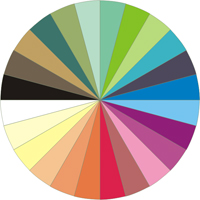
\includegraphics[scale=0.9]{logo.jpg} \\[1cm]
\HRule \\[0.4cm]
{ \huge \bfseries IntelliPhoto \\[0.15cm] }
\HRule \\[1.5cm]
Gruppe 3
\\[1cm]
\today \\ [1cm]
\end{titlepage}


\tableofcontents
\newpage

%%%%%%%%%%%%%%%%%%%%%%%%%%%%%%%%%%%%%%%%%%%%%%%%%%%%%%%%%%%%%%%%%%%%%%%%%%%%%%%%%%%%%%%%%%%%%%%%

\section{Einleitung}

\subsection{Grundsätzliches}
IntelliPhoto ist ein Bild Editor der von unserer Gruppe im Rahmen des Software Engineering Praktikum im Wintersemester 2019/20 entworfen und programmiert wurde. Ziel des Praktikum war es sich mit den Schritten der heutigen Software Entwicklung auseinander zu setzen und erste Erfahrungen in diesem Bereich zu sammeln. Betreut wurde das Projekt von Prof. Janet Sigmund und Shadi Saleh.\\
\\
Im folgenden sind die einzelnen Schritte des Softwarelebenszyklus für IntelliPhto dokumentiert.
Orientiert wird sich dabei an der das Praktikum begleitenden Vorlesung Software Engineering an der TU Chemnitz. Definitionen werden wenn nicht anders vermerkt dieser Vorlesung entnommen.
\begin{figure}[H]
  \centering
  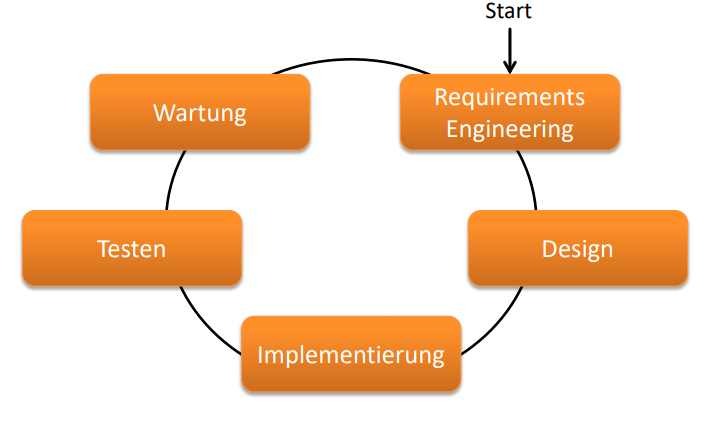
\includegraphics[width=\textwidth,frame]{Softwarezyklus.png}
	\caption{Softwarelebenszyklus nach Vorlesung}
	\label{fig1}
\end{figure}
\noindent
Es ist sinnvoll sich an diesen Zyklus zu halten, weil dadurch Probleme frühzeitig erkannt und behoben werden können. Die Kosten ein Problem zu beheben stiegen mit Fortschritt des Projekts.

\subsection{Anforderungsbeschreibung}
IntelliPhoto liegt die folgenden Anforderungsbeschreibung, in der die Grundfunktionen des Editor spezifiziert werden, zu Grunde. Im Laufe des Projektes kamen weitere Wünsche und Anforderungen von "Kunden" \, hinzu. Diese werden an entsprechender Stelle vorgestellt.\\ 

\begin{figure}[H]
  \centering
  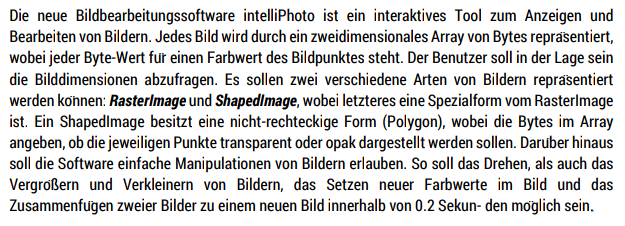
\includegraphics[width=\textwidth,frame]{Anforderungsbeschr.png}
	\caption{Anforderungsbeschreibung IntelliPhoto}
	\label{fig2}
\end{figure}
\noindent
Diese Beschreibung bildet den Kern des Projekts und wird im folgenden immer als Anforderungsbeschreibung referenziert. Auf Sie wird, insbesondere im Design und Requirements Engineering Abschnitt, oft verwiesen. 


%%%%%%%%%%%%%%%%%%%%%%%%%%%%%%%%%%%%%%%%%%%%%%%%%%%%%%%%%%%%%%%%%%%%%%%%%%%%%%%%%%%%%%%%%%%%%%%%
	
	
\section{Requirements Engineering} 

\subsection{Motivation}
Requirements beschreiben Bedingungen oder Eigenschaften, die ein System benötigt um Probleme zu lösen, Ziele zu erfüllen oder ein einen Vertrag/Standard zu genügen. Sie werden an ein Programm gestellt und spezifizieren dessen Eigenschaften und Funktionalitäten. Bestimmt werden Sie von den Stakeholdern, dieser Begrifft bezeichnet die Gruppen die Interesse am Projekt hegen.\\
\\
Requirements Engineering bezeichnet den Vorgang, diese Requirements zu finden und zu kategorisieren. Es ist ein wichtiger Schritt beim Software-Entwurf da eine eindeutige und überprüfbare Anforderungsbeschreibung entsteht. Es ist somit möglich Widersprüche zu identifizieren und eine vom Kunden eventuell in Fachsprache verfasste Beschreibung verständlich zu gestalten. 

\subsection{Volere-Snow-Cards} 
Requirements Engineering glieder sich in vier Schritte: Anforderungsermittlung, Anforderungsanalyse, Anforderungsbeschreibung und Anforderungsrevision. Bei der Anforderungsermittlung werden Stakeholder- und Szenario basiert die Requirements identifiziert. In der folgenden Anforderungsanalyse werden diese in Funktionale, \textit{was} soll das System leisten, und nicht-Funktionale, \textit{wie} solle das System etwas leisten, Requirements unterteilt, sowie deren Erfüllbarkeit überprüft und Prioritäten zugeordnet. Die Anforderungsbeschreibung fasst obige Ergebnisse in genormter Form zusammen, in unserem Projekt nutzen wir dazu das Format der Volere-Snow-Card. Diese Beschreibung wird in der Anforderungsrevision erneut auf Probleme und Realisierbarkeit geprüft.\\
Im folgenden finden sich unsere Ergebnisse dieser Schritte als Volere-Snow-Cards: 
\\
\\
\textbf{@TODO Volere Snow Cards}\\
eventuell auch in Anhang


%%%%%%%%%%%%%%%%%%%%%%%%%%%%%%%%%%%%%%%%%%%%%%%%%%%%%%%%%%%%%%%%%%%%%%%%%%%%%%%%%%%%%%%%%%%%%%%%


\section{Design}
Generelles Ziel ist es eine Struktur zu finden die einfach zu verstehen und zu implementieren ist, Möglichkeiten zur Erweiterung bietet und wenn korrekt implementiert die Realisierung aller Anforderungen garantiert. Die Idee ist dabei das Programm in einzelne miteinander interagierende aber von einander unabhängige Objekte aufzuteilen und diesen Funktionen zuzuweisen. Dies nennt man Objekt-Orientiertes Dekomposition und wurde von uns beim designen des Programms verwendet. Es sei angemerkt dass dies ein iterativer Prozess ist, sich also Ergebnisse auch nach der Design Phase ändern können. Im folgenden finden sich also unsere finalen Ergebnisse zum Zeitpunkt der Abgabe.

\subsection{Responsibility-Driven Design}
Eine Technik ein Objekt-Orientierten Designs zu realisieren ist mittels Responsibility-Driven Design (RRD). Das RRD gliedert sich in eine initiale Exploration, bei der Klassen, Verantwortlichkeiten und  Kollaborationen identifiziert werden, und eine detaillierte Analyse, bei der Ergebnisse konkretisiert werden und nach Klassenhierarchien gesucht wird um Klassen eine vollständige Signatur zu geben.\\
Die Ergebnisse der ersten Phase können mit CRC-Karten (stellvertretend für Candidates-Responsibility-Collaboration-Karten) einheitlich visualisiert werden. In unserem Fall erhalten wir folgende Karten:\\
\\
\textbf{@TODO CRC-Karten}\\


\begin{figure}
\centering
\begin{subfigure}{.5\textwidth}
  \centering
  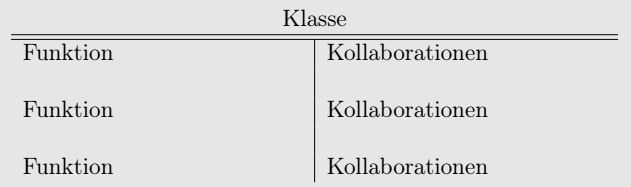
\includegraphics[width=.95\linewidth,height=2.5cm]{CRC.png}
  \caption{A subfigure}
  \label{fig:sub1}
\end{subfigure}%
\begin{subfigure}{.5\textwidth}
  \centering
  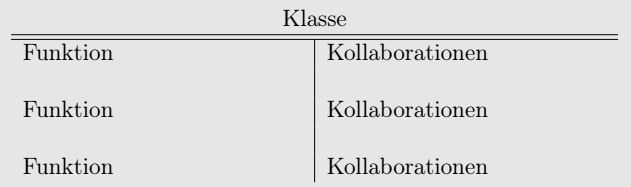
\includegraphics[width=.95\linewidth,height=2.5cm]{CRC.png}
  \caption{A subfigure}
  \label{fig:sub2}
\end{subfigure}
\caption{A figure with two subfigures}
\label{fig:test}
\end{figure}


Die Ergebnisse nach der detaillierten Analyse können auf verschiedene Weise dargestellt werden. Die Informationen die für eine vollständige Signatur benötigt werden können etwa auf der Rückseite der jewiligen CRC-Karte vermerkt werden\footnote{siehe https://de.wikipedia.org/wiki/Class-Responsibility-Collaboration-Karten}. Klassenhierarchien können zum Beispiel mit Venn Diagrammen abgebildet werden. Eine Möglichkeit die beiden Informationen in einem gemeinsamen Diagramm vereint darstellt, ist das im nächsten Absatz für unser Projekt vorgestellte UML-Klassendiagramm. 

\subsection{UML-Diagramme}
UML (Unified Modeling Language) repräsentiert den internationalen Industriestandard für grafische Modellierungssprache. Sie ermöglicht komplexe Designs in Form von Diagrammen zu visualisieren.
Der große Vorteil an UML ist das es hinreichend gut dokumentiert und standardisiert ist, dass heißt dass Diagramme ohne gesonderte Erklärung der Bedeutung ihrer Symbole verständlich sind sofern Sie dem UM-Standard genügen. Sollte der Betrachter mit diesem nicht vertraut sein ist es ein einfaches für ihn die Bedeutung heraus zu finden. Deshalb wird im folgenden auf Erklärung der Diagramme verzichtet da diese dem Standard genügen.  

\subsubsection{Klassen-Diagramm}
Das vermeintlich wichtigste UML-Diagramm ist das Klassendiagramm, da in diesem kompakt alle Klassen mit ihrer Signatur und alle Interaktionen abgebildet werden können. Unserer UML-Diagramm für IntelliPhoto basiert auf der detaillierten Analyse, dem zweiten Schritt des vorhergegangenen RDD.\\
\\
\textbf{TODO UML Klassen Diagramm machen}
\\

\subsubsection{Use-Case Diagramm}
Auch können mit UML Use-Case Diagramme erstellt werden. Ein Use-Case ist eine generische
Beschreibung einer gesamten Transaktion, welche mehrere Aktoren involviert. Ein Use-Case Diagramm präsentiert eine Menge von Use-Cases (Ellipsen) und deren externe Aktoren, die mit dem System interagieren. Das Anwendungsverhalten verschiedener Nutzer Gruppen ist uns wie folgt gegeben worden:
\begin{figure}[H]
  \centering
  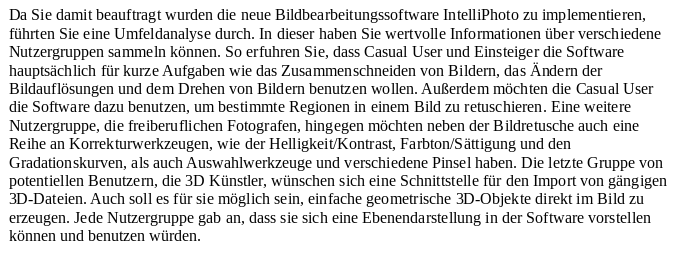
\includegraphics[width=\textwidth, height=5.5cm, frame]{usecaseanalyse.png}
	\caption{Ergebnisse für Anwendung Intelli Photo}
	\label{fig1}
\end{figure}
\noindent
Durch verarbeiten dieser Informationen kommen wir zu folgenden exemplarischen zwei Use-Case Diagrammen für IntelliPhoto:\\
\\
\textbf{@TODO Use Case Diagramme}
\\

\subsubsection{Sequenz Diagramme}
Ein Szenario ist eine Instanz von einem Use Case, das ein typisches Beispiel einer Ausführung zeigt.
Szenarien können durch UML Sequenzdiagramme dargestellt werden. Ein Sequenzdiagramm beschreibt ein Szenario durch das Zeigen von Interaktionen zwischen einer Menge von Objekten in einer zeitlichen Abfolge. Objekte (keine Klassen!) werden als vertikale Balken gezeichnet. Events oder Nachrichtensendungen werden als horizontale (oder schräge) Pfeile vom Sender zum Empfänger gezeichnet. Im folgenden zeigen wir zwei Sequenz Diagramme für IntelliPhoto. Im ersten ist das Diagramm für das Szenario X, im zweiten für das Szenario Y dargestellt.\\
\\
\textbf{@TODO Sequenz Diagramme}
\\

\subsubsection{Zustandsdiagramm}
Ein Zustandsdiagramm beschreibt die zeitliche Evolution eines Objektes von einer gegebenen Klasse
in Abhängigkeit von Interaktionen mit anderen Objekten innerhalb und außerhalb des Systems.\\
Im folgenden ist exemplarisch das Zustandsdiagramm für ein Objekt der Klasse x und ein Objekt der Klasse y dargestellt.\\
\\
\textbf{@TODO 2 Zustandsdiagramme}
\\


%%%%%%%%%%%%%%%%%%%%%%%%%%%%%%%%%%%%%%%%%%%%%%%%%%%%%%%%%%%%%%%%%%%%%%%%%%%%%%%%%%%%%%%%%%%%%%%%


\section{Implementierung}
\subsection{Programmiersprache und Libraries}
Wir haben uns bei der Implementation von IntelliPhoto für die Programmiersprache C++ entschieden. C++ bietet die Möglichkeit zum Objekt orientierten Programmieren was ein für uns nach der Designphase (mit Objekt orientierte Dekomposition) ein essentielles Programmierparadigma war. C++ bietet weiterhin die Vorteile dass es Plattform unabhängig ist, über eine starke Community, im Sinne von vielen Libraries und Foren, verfügt und eine sehr performante Sprache ist. Letzteres war insbesondere im Anbetracht der Zeit-Constraints in der Anforderungsbeschreibung ein wichtiger Grund für die Entscheidung. Das einzige Problem dass C++ mit sich bringt ist dass es keinen Garbage Collector besitzt, es kann also durch unaufmerksames Programmieren schnell viel Speicher von der Anwendung benötigt werden.\\
\\
Die Kern Library unseres Programms ist Qt5. Qt ist ein open source Anwendungsframework und GUI-Toolkit zu plattformübergreifenden Entwicklung von Programmen. Grund für diese Entscheidung war zunächst die gute Kompatibilität mit C++, so ist Qt in dieser Sprache implementiert und setzt selbst einen Objekt orientierten Ansatz um. Zum anderen wird Qt stark in real Welt Anwendungen genutzt, etwa beim KDE-Plasma \footnote{https://en.wikipedia.org/wiki/Qt\_(software)\# Qt\_ in\_ use}. Die für uns letztlich wichtigsten Faktoren für die Entscheidung waren die Existenz einer Qt eigene Wikipedia  \footnote{https://wiki.qt.io/Main} und die mit 'Qt Creator' frei verfügbare IDE speziell für die Entwicklung mit Qt. Beides war für uns als Neulinge in der GUI-Programmierung sehr hilfreich und hat dazu beigetragen, dass wir das Projekt umsetzen konnten.

\subsection{Doxygen Code Dokumentation?}
Wär echt nice zu haben
%%%%%%%%%%%%%%%%%%%%%%%%%%%%%%%%%%%%%%%%%%%%%%%%%%%%%%%%%%%%%%%%%%%%%%%%%%%%%%%%%%%%%%%%%%%%%%%%


\section{Testen}
\subsection{Test Resultate}
Im folgenden finden sich unsere Testresultate. Wir haben uns dafür entschieden folgende Arrten von Tests durchzuführen....\\
\textbf{@TODO Testresultate}

\subsection{Bekannte Fehler und Probleme}
Die folgenden Bugs und anderer Probleme sind bekannt und werden bei Abgabe des Projektes noch nicht behoben sein....\\
\textbf{@TODO Bugs und Probleme}


%%%%%%%%%%%%%%%%%%%%%%%%%%%%%%%%%%%%%%%%%%%%%%%%%%%%%%%%%%%%%%%%%%%%%%%%%%%%%%%%%%%%%%%%%%%%%%%%


\section{Wartung}
Da IntelliPhoto im Rahmen eines Vorlesung begleitenden Praktikums erstellt wurde, also keine Veröffentlichung des Programms und damit reale Nutzung geplant sind, sowie die Verantwortlichkeiten der Gruppenmitglieder mit Abgabe des Projektes enden, ist es nicht geplant Wartungstätigkeiten auszuführen. Dies soll jedoch keines Falls bedeuten diese wäre in einem anderen Szenario nicht notwendig. Uns ist klar, dass eine Wartung des Programmes allein wegen der bereits bekannten Fehler vonnöten wäre, die im Rahmen des Projektes nicht behoben werden konnten. Außerdem hat das Programm mit hoher Wahrscheinlichkeit eine Vielzahl, trotz testen, noch unbekannter Fehler, die erst in der extensiven Nutzung erkannt und gewartet werden müssten.  

%%%%%%%%%%%%%%%%%%%%%%%%%%%%%%%%%%%%%%%%%%%%%%%%%%%%%%%%%%%%%%%%%%%%%%%%%%%%%%%%%%%%%%%%%%%%%%%%

\section{Schlusswort}
IntelliPhoto ist das erste größere Software Projekt an dem jedes unserer Gruppenmitglieder gearbeitet hat. Uns ist bekannt dass das Resultat viel zu wünschen übrig lässt und vieles nicht so funktioniert wie es sollte. Dennoch haben wir, gerade aus der Menge unserer Fehler, eine Menge gelernt und sind recht zufrieden mit dem Ergebnis, für ein erstes Projekt.\\
\\
Viel Spaß mit dem Programm,\\
\center{Pascal Schröter, Jeremias Piljug, Dongze Yang und Xiangyu Tong}
\center{Gruppe 3}


\end{document}
